\documentclass[12pt,a4paper]{article}
\usepackage[utf8]{inputenc}
\usepackage[T1]{fontenc}
\usepackage[french]{babel}
\usepackage{hyperref}
\usepackage{enumitem}
\usepackage{geometry}
\usepackage{amsmath}
\usepackage{datetime}
\usepackage{graphicx}
\usepackage{amsmath}
\usepackage{amssymb}
\usepackage{tikz}
\usetikzlibrary{calc}
\usetikzlibrary{arrows.meta, positioning, fit, backgrounds, shapes.geometric, decorations.pathreplacing}


\geometry{margin=2.5cm}
\usepackage{graphicx}
\title{Coordination et exactitude dans les systèmes distribués\\[1em]
\large Histoire et Épistémologie de l'Optimisation}
\author{Hugo RAMILLON \and Adam NAJI \and Eduard DICONI}
\newdate{date}{24}{03}{2026}
\date{\displaydate{date}}

\begin{document}
\maketitle
\thispagestyle{plain}
\begin{figure}[h]
    \centering
    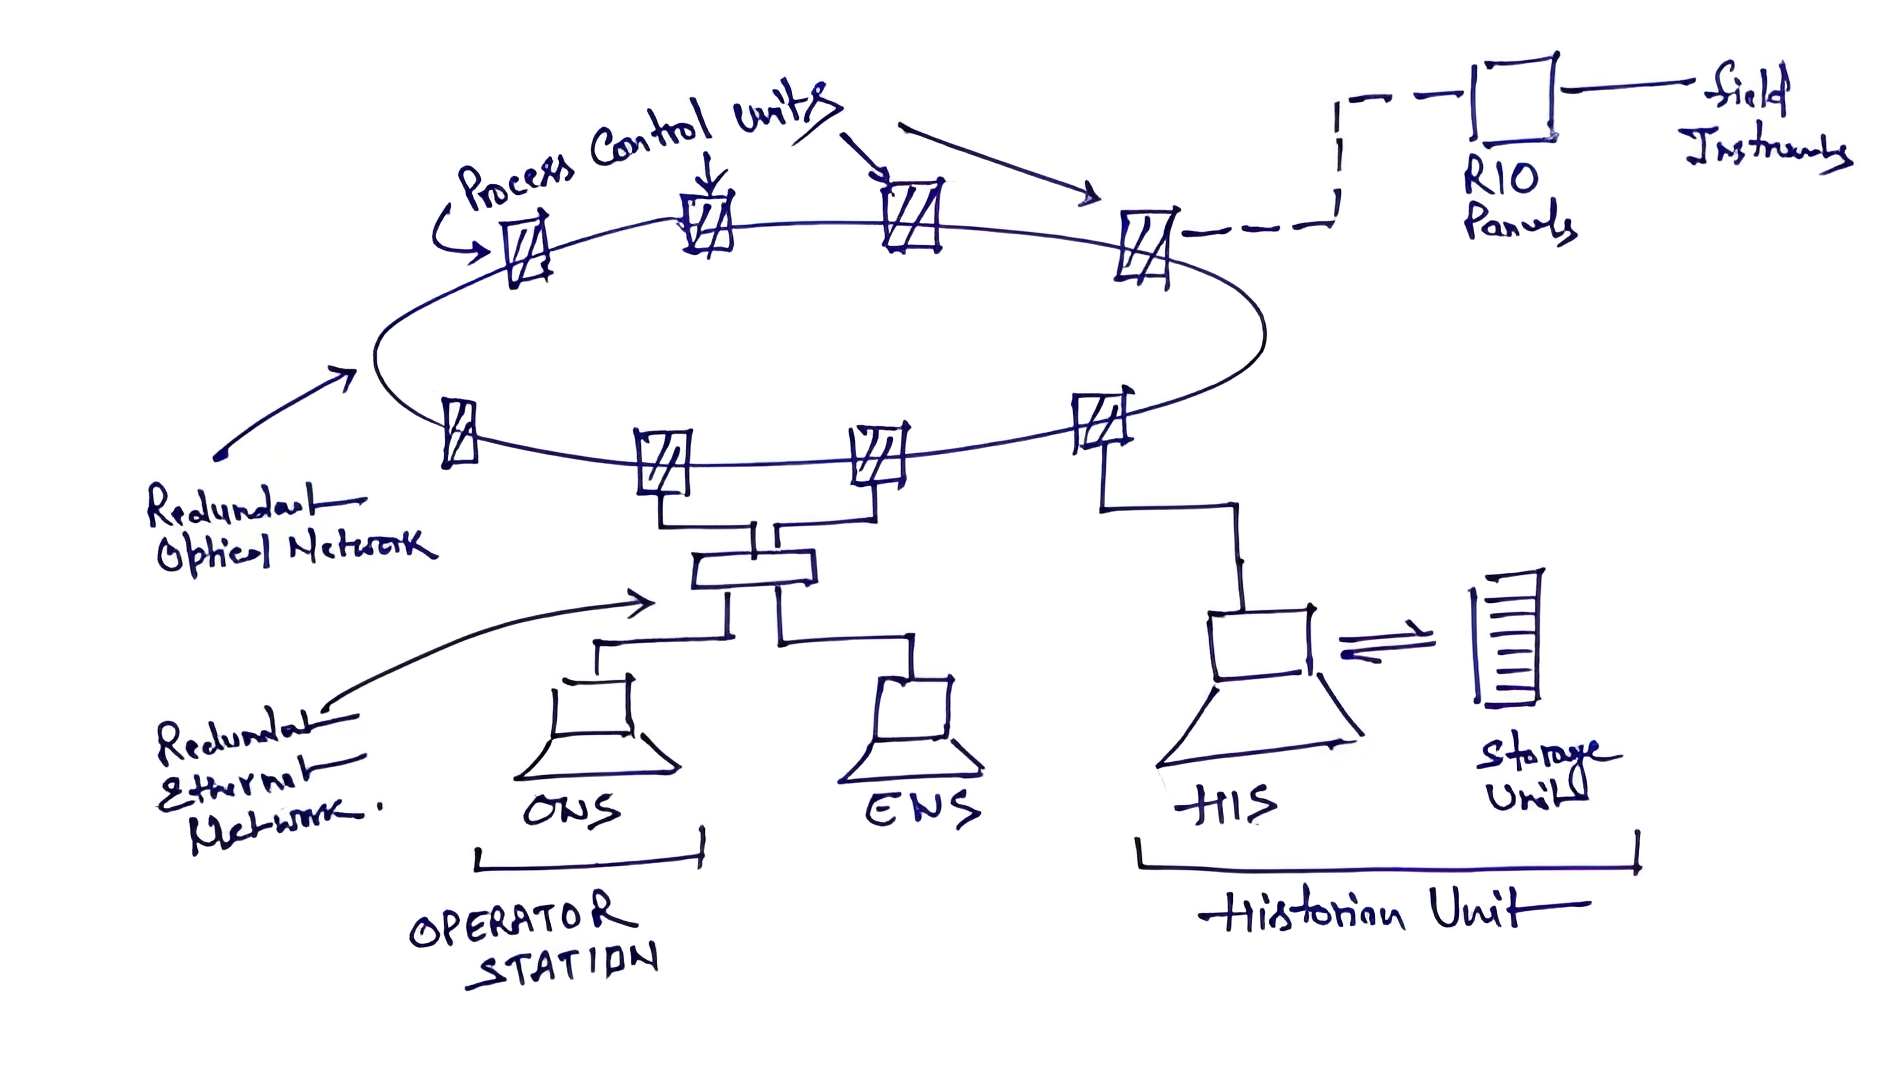
\includegraphics[width=1\linewidth]{fig_0_cover.png}
    \label{fig:placeholder}
\end{figure}



\newpage

\tableofcontents
% citer + de ref askip il en maque %
\newpage
\section{Introduction}

En juillet 1997, le rover Mars Pathfinder \cite{MarsPathfinder}, le premier à opérer en dehors du système Terre-Lune, semble avoir un problème critique: il redémarre en boucle. C'est la fin d'une mission de haute importance pour la NASA. Du moins c'est ce que l'on a cru : le problème était logiciel, la priorité des tâches données au robot était inversée, en d'autres termes des tâches considérées comme peu importantes étaient bloquées, ce qui faisait redémarrer le robot en boucle. Cet exemple nous montre plusieurs choses. L'importance de la coordination; les tâches doivent communiquer clairement et se coordonner pour partager une ressource. La notion de vérité peut être locale, chaque tâche possède une vérité locale cohérente mais qui peut être contradictoire avec les autres. Le système échoue parce qu'il n'a pas de vérité globale sur son état.

Pour parler de façon générale des systèmes distribués, nous pouvons écouter les propos de Bernadette Charron-Bost \cite{CharronBost}, informaticienne spécialisée dans les systèmes distribués et primée par l'académie des sciences en 2019. Lors d'une interview au CNRS, elle définit un système distribué comme \textit{"Toutes sortes de systèmes [\ldots] formés d'entités indépendantes qui communiquent via un médium"}.

Dans un système distribué, la \textbf{coordination} désigne la manière dont plusieurs composants --- souvent appelés nœuds --- parviennent à organiser leurs actions pour accomplir une tâche commune. Elle repose sur des échanges de messages, des synchronisations ou des protocoles qui permettent aux nœuds d'agir de façon cohérente malgré leur autonomie.

La notion de \textbf{vérité}, elle, est beaucoup plus délicate. Dans un système distribué, aucun nœud ne possède l'ensemble des informations: chacun ne voit qu'une partie du système et construit donc sa propre "vérité locale", basée sur ce qu'il sait à un instant donné. Or ces vérités locales peuvent être incomplètes, décalées dans le temps, voire contradictoires entre elles lorsque la communication est lente ou incertaine.

Cette tension est au cœur du sujet: d'un côté, les nœuds doivent pouvoir décider de ce qui est vrai pour agir; de l'autre, ils n'ont jamais accès à une vérité globale immédiate de cette manière. Comment définir une vérité commune dans un système où chaque composante évolue de manière indépendante et ne possède qu'une vision partielle du monde?

Pour y répondre nous verrons en quoi précisément les systèmes distribués sont vecteurs d'incertitude via des mécaniques qui leur sont internes et qui sont compliqués à détourner. Puis nous verrons quelles sont les solutions que les chercheurs ont trouvées pour tenter de mettre fin à cette incertitude qui plane au dessus de ces systèmes. Finalement nous en verrons les limites et les craintes que nous pouvons avoir dessus au vu de l'utilisation des systèmes distribués dans le monde.





% %
% --- PARTIE EDWARD --- % 
% %
\newpage
\section{Incertitude dans les systèmes distribués}

Comme dit en introduction, les nœuds des systèmes distribués observent uniquement une partie locale du monde, le tout avec des horloges désynchronisées. On cherche à comprendre toute la complexité du problème dans cette partie.



\subsection{Une incertitude qui provient de l'essence des machines déterministes}


Martin Kleppmann, chercheur en systèmes distribués à l'Université de Cambridge et ex-ingénieur informatique chez LinkedIn, consacre le huitième chapitre de son ouvrage \textit{Designing Data-Intensive Applications} \cite{Kleppmann2017}. aux difficultés inhérentes aux systèmes distribués. Contrairement à un programme exécuté sur une machine isolée, qui produit un résultat déterministe pour des entrées de données, un système distribué introduit une dimension d'incertitude fondamentale.

\vspace{0.25cm}
Sur une machine unique, un programme compilé s'exécute de manière prévisible et répétable : à entrées identiques, résultats identiques. Un algorithme de tri, par exemple, produira toujours la même séquence ordonnée pour un ensemble de valeurs donné. Cela va sans dire que cette prévisibilité repose sur l'hypothèse que la machine fonctionne correctement : mais nous ne rentrerons pas dans les détails de cette hypothèse, car cela rentre plus dans le cadre de l'électronique et du matériel, comme par exemple la mémoire-vive ECC ou la nature inconsistante de notre stockage (HDD et erreurs de lecture, SSD et nombre de lectures fini, média optiques qui peuvent périr avec le temps...).

\vspace{0.25cm}
Les systèmes distribués, eux, bouleversent cette logique déterministe. Kleppmann distingue deux contextes où la distribution s'impose : le calcul haute performance (HPC), où une tâche intensive est répartie entre plusieurs machines locales qui doivent se coordonner, et le réseau (networking), où des machines distantes communiquent via des canaux imparfaits comme Internet, le Wi-Fi ou le Bluetooth. Dans ces environnements, l'ajout de la distribution transforme un système déterministe en système non-déterministe : les délais de communication deviennent imprévisibles, les messages peuvent être perdus, et les horloges locales dérivent indépendamment \cite[p.~274]{Kleppmann2017}.

\vspace{0.25cm}
Cette transformation pose une question centrale : comment garantir la cohérence du système lorsque la communication elle-même est incertaine et que les données peuvent être fausses ou obsolètes? Kleppmann identifie trois sources majeures d'incertitude : les réseaux non-fiables, les horloges désynchronisées, et les pauses imprévisibles des processus.

\vspace{0.25cm}
Ensemble, ces facteurs rendent impossible toute garantie absolue sur l'état global du système.

\subsection{Des nœuds dont les paramètres communs restent désynchronisés}

Dans un système distribué, chaque nœud exécute un comportement local déterministe, mais il évolue dans un environnement où les informations externes , notamment les messages provenant d’autres nœuds , arrivent avec des délais imprévisibles. Cette dissociation entre déterminisme local et incertitude globale rend problématique toute tentative de coordination fondée sur des paramètres supposés communs, comme un ordre temporel partagé. Lamport montre que cette difficulté est structurelle : dans un système distribué, il n’existe pas de notion de temps global implicite permettant d’ordonner sans ambiguïté l’ensemble des événements \cite{Lamport1978}. L’ordre des événements ne peut être défini qu’à partir de ce qui est effectivement observable par les processus.

\subsubsection{Introduction du temps dans les nœuds d'un système distribué}

Pour formaliser cette observabilité limitée, Lamport introduit la relation dite \emph{happened-before}. Intuitivement, cette relation exprime une dépendance causale minimale entre événements. Lorsqu’un même processus exécute deux actions successives, l’ordre de ces actions est connu localement. De même, lorsqu’un processus envoie un message et qu’un autre le reçoit, l’envoi précède nécessairement la réception. En revanche, si deux événements surviennent sur des processus distincts sans qu’aucune chaîne de messages ne les relie, alors aucun des deux processus ne peut déterminer lequel est antérieur à l’autre. La relation \emph{happened-before} capture exactement ces situations : elle formalise ce qui peut être déduit de l’exécution locale et des communications effectives, sans introduire d’hypothèses supplémentaires sur le temps.

Cette formalisation met en évidence une limite fondamentale : l’ordre ainsi défini est seulement partiel. L’existence d’événements concurrents — c’est-à-dire non comparables — n’est pas un défaut du modèle, mais la conséquence directe de la distribution. Même si, dans le monde physique, un événement a eu lieu avant un autre, cette information n’est pas accessible aux nœuds tant qu’aucun mécanisme explicite ne la transmet. Ainsi, la simple notion d’ordre causal ne suffit pas à synchroniser globalement les paramètres du système. Elle décrit fidèlement ce que les nœuds peuvent savoir, mais révèle en même temps l’impossibilité d’une coordination temporelle parfaite fondée uniquement sur l’échange de messages. Cette problématique peut encore être observable : le 1er août 2012, le Knight Capital déploie du code pour faire des ordres de trading sur différents serveurs, leurs logiques étant différentes et leurs ordres pas tous connus les uns les autres. Les serveurs ont fait des ordres illogiques amenant à perdre près de 450 millions de dollars en 45 minutes. Même si, dans le monde physique, un événement a eu lieu avant un autre, cette information n’est pas accessible aux nœuds.

\subsubsection{Introduction d'horloges et désynchronisation avec le monde physique}

Cette difficulté ne disparaît pas lorsque l’on cherche à introduire des horloges physiques afin de reconstruire une référence temporelle commune. Cristian étudie précisément ce problème en considérant des systèmes distribués dans lesquels les processus tentent de synchroniser leurs horloges à l’aide d’échanges de messages \cite{Cristian1989}. Le point central est que le délai de transmission d’un message n’est ni constant ni entièrement prévisible : un processus ne peut jamais savoir combien de temps un message a effectivement passé dans le réseau. Par conséquent, lorsqu’un nœud ajuste son horloge à partir d’une information temporelle reçue, cette information est déjà potentiellement obsolète. Cristian tente alors de répondre à la question en introduisant des bornes statistiques sur les délais, ce qui permettrait d'atténuer une certaine désynchronisation des systèmes.

\vspace{0.25cm}

Même en supposant l’existence de bornes statistiques sur les délais, la synchronisation obtenue reste fondamentalement approximative. Les protocoles analysés par Cristian ne peuvent garantir qu’un écart borné entre horloges, souvent exprimé de manière probabiliste, et uniquement sous des hypothèses fortes sur le comportement du réseau. En particulier, ils ne permettent pas d’établir une égalité stricte entre les horloges des nœuds, mais seulement de limiter leur dérive relative. Ainsi, l’introduction d’horloges physiques ne supprime pas l’incertitude temporelle : elle la transforme en une incertitude contrôlée, mais toujours présente.

\vspace{0.25cm}

Cette observation renforce le constat établi par Lamport : l’absence d’un temps global fiable n’est pas un artefact du modèle logique, mais une contrainte intrinsèque des systèmes distribués réels. Même lorsque l’on enrichit le système avec des mécanismes temporels explicites, les paramètres supposés communs restent nécessairement désynchronisés, ce qui interdit toute coordination fondée sur une chronologie parfaitement partagée.

\subsubsection{Conséquences dans le monde réel}

Les conséquences de cette désynchronisation apparaissent de façon particulièrement nette dans la mise en œuvre de services distribués critiques. L’approche des machines à états répliquées, étudiée dans le SMSurvey \cite{Schneider1990}, repose sur l’hypothèse que plusieurs nœuds peuvent maintenir un service cohérent à condition de traiter exactement la même séquence de requêtes dans le même ordre. Or, cette exigence suppose précisément un accord global sur l’ordre des événements, accord que le système distribué ne fournit pas naturellement. La nécessité de mécanismes complexes pour imposer cet ordre montre que la désynchronisation des paramètres — temporels ou logiques — a des conséquences directes sur la cohérence, la fiabilité et la tolérance aux pannes des systèmes distribués. De cette façon, le 30 juin 2012, une seconde intercalaire doit être ajoutée à tous les serveurs pour recaler les horloges avec la rotation réelle de la Terre au temps UTC(23:59:60). Cependant les ordres ne sont pas reçus, ou au mauvais moment : cela entraîne des désynchronisations mondiales se passent sur tous les serveurs du monde. Les serveurs de Reddit par exemple sont indisponibles pendant plusieurs heures, ce sera aussi le cas de nombreux serveurs autour du monde.

\vspace{0.25cm}

Ainsi, malgré les efforts déployés pour reconstruire artificiellement un ordre ou une synchronisation, les nœuds d’un système distribué opèrent fondamentalement sur des informations locales et désynchronisées. Cette contrainte structurelle impose des compromis inévitables entre coordination, performance et robustesse, et constitue l’un des obstacles majeurs à l’établissement d’une vérité globale partagée dans les systèmes distribués.

\subsection{De la connaissance de l'état des autres machines du réseau}

De cette façon, nous voyons bien qu'il est compliqué pour les nœuds d'un réseau d'être correctement synchronisés. Il s'ajoute à cette difficulté la capacité à connaître l'état dans lequel les autres nœuds se trouvent. Si tel ou tel nœud se retrouve déconnecté alors comment doit-on réagir et s'adapter. On voit bien que cela pose un autre problème, celui de la connaissace de l'etat interne des noeuds du réseau sans savoir s'ils peuvent communiquer ou communiquer correctement.

Dans un système distribué, la communication réseau introduit une incertitude fondamentale. Lorsqu'un nœud envoie une requête et n'obtient pas de réponse, il est impossible de déterminer avec certitude la cause du silence : soit la requête n'a jamais atteint le destinataire, soit le nœud distant est effectivement en panne, soit la réponse a été perdue en chemin \cite[p.~278]{Kleppmann2017}.

\begin{figure}[h]
    \centering
    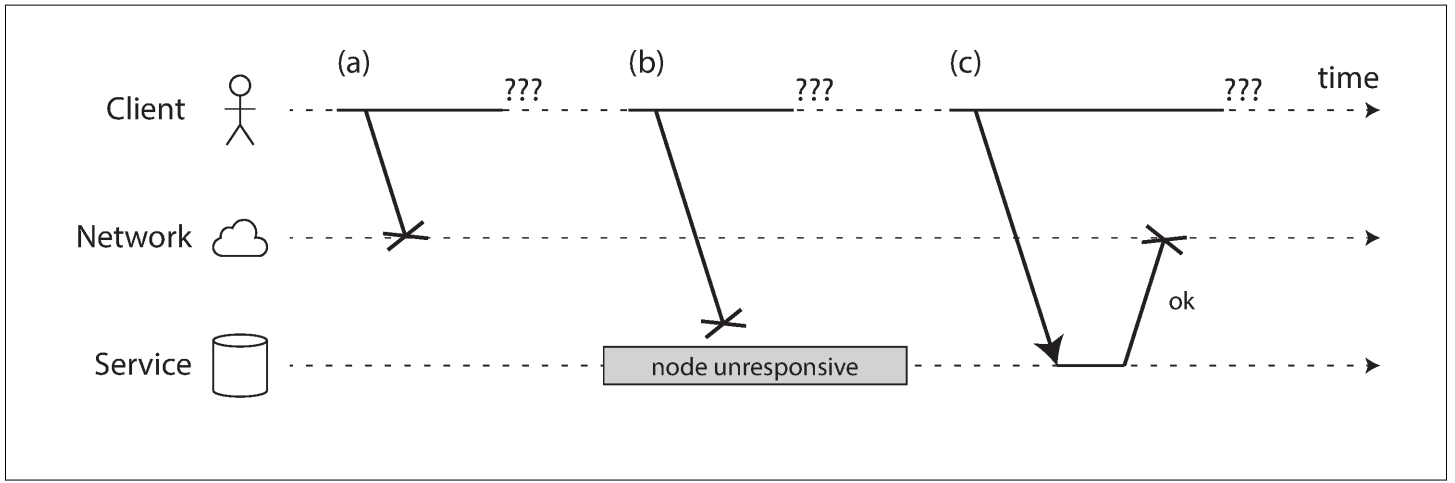
\includegraphics[width=0.8\linewidth]{fig_2_2_networkuncertainty_mklep.png}
    \caption{Si vous envoyez une requête et ne recevez pas de réponse, il est impossible de distinguer si (a) la requête a été perdue, (b) le nœud distant est hors service, ou (c) la réponse a été perdue. \cite[p.~278]{Kleppmann2017}}
    \label{fig:network-uncertainty}
\end{figure}

\subsubsection{Le temps d'attente est-il un problème de long délai ou de crash d'un nœud ?}

Dans un système distribué, observer un autre nœud comme “mort” ou “vivant” n’est jamais immédiat, car cette observation dépend de la réception de messages sur le réseau. Chandra et Toueg introduisent l’abstraction des « failure detectors » pour formaliser cette difficulté : chaque nœud possède un composant local qui émet des suspicions sur l’état des autres nœuds, c’est-à-dire s’ils sont encore actifs ou s’ils se sont arrêtés (crash). Cependant, ces détecteurs sont intrinsèquement « unreliable » (non fiables) : ils peuvent suspecter à tort un nœud correct ou, inversement, ne pas suspecter immédiatement un nœud qui a effectivement crashé.

\vspace{0.25cm}

Cette imprécision n’est pas simplement “un bug” : elle exprime l’impossibilité fondamentale de distinguer, dans un système asynchrone, un nœud qui est très lent (du fait de longs délais réseau) d’un nœud qui est réellement tombé en panne. Tant qu’un message de “je suis vivant” ne parvient pas, le nœud distant peut être correct mais simplement lent ; déclarer mort un nœud correct est alors une fausse accusation du détecteur. Et même lorsqu’un nœud a réellement crashé, il peut ne pas être suspecté immédiatement et durablement, car aucun délai maximum sur la livraison des messages n’est garanti dans un système distribué asynchrone.

\vspace{0.25cm}

Du point de vue pratique, cela signifie que le simple fait d’attendre un certain temps sans réponse ne permet jamais de savoir avec certitude si l’absence de réponse est due à un délai très long ou à un crash effectif. C’est pourquoi Chandra et Toueg définissent des détecteurs qui peuvent se tromper un nombre arbitraire de fois, et seulement au bout d’un certain temps suffisamment long peuvent garantir de ne plus faire d’erreur pour des décisions critiques comme le consensus.

\vspace{0.25cm}

Concrètement, cette incertitude a des conséquences directes : si un nœud attend une réponse et ne sait pas si l’autre nœud est juste ralenti ou réellement tombé, il ne sait pas s’il doit répéter la requête, basculer sur une autre copie du service, ou considérer l’autre nœud comme définitivement indisponible. Ce problème de connaissance d’état — savoir si un nœud distant est vivant ou crashé — est l’un des défis centraux de la tolérance aux pannes dans les environnements distribués. Dans les systèmes réels, cette difficulté se traduit par des mécanismes complexes de redondance, de temps d’attente adaptatifs, et de consensus distribué qui doivent être conçus en tenant compte de ces limitations fondamentales plutôt qu’en supposant qu’une absence de réponse implique toujours une panne.

\subsubsection{Capacité à prendre une décision lorsque un nœuds tombe en panne}

Cette impossibilité de distinguer un nœud très lent d’un nœud ayant subi une panne a des conséquences théoriques profondes. Fischer, Lynch et Paterson montrent dans leur résultat fondamental que, dans un système distribué asynchrone, il est impossible de garantir un consensus déterministe dès lors qu’un seul processus peut tomber en panne \cite{FLP1985}. Leur démonstration repose précisément sur l’absence de borne supérieure connue sur les délais de communication : un processus peut toujours hésiter à décider, car un message attendu pourrait encore arriver ultérieurement, ou bien ne jamais arriver du fait d’un crash.

Ainsi, même si tous les processus corrects suivent scrupuleusement l’algorithme, l’incertitude entre retard et panne empêche toute progression garantie du système. Ce résultat formalise l’idée que le problème n’est pas algorithmique, mais informationnel : aucun mécanisme purement distribué ne permet de lever cette ambiguïté dans un modèle asynchrone. Le théorème FLP établit donc une limite fondamentale à la connaissance de l’état global du système et motive l’introduction d’hypothèses supplémentaires, telles que des détecteurs de fautes ou des hypothèses de synchronisme partiel, pour contourner cette impossibilité.
% %
% --- FIN PARTIE HUGO --- % 
% %






\newpage
\section{Implémentation de mécanismes de coordination, établir une vérité générale en systèmes distribués}

Comme la vérité en système distribué semble être locale, elle doit donc être construite via différentes solutions permettant de comprendre le système global. Plusieurs solutions existent: consensus, cohérence, ordonnancement global.

\subsection{Résoudre le problème du temps entre les nœuds du système}

L'un des obstacles à la coordination dans un système distribué est la notion de temps entre les nœuds comme on a vu dans la partie précédente, des solutions nouvelles ont été trouvées à travers le temps.

\subsubsection{Les principes trouvés par Lamport}

Comme vu dans la première partie, Lamport observe que les horloges physiques ne permettent pas d’obtenir une synchronisation fiable dans un système distribué : les dérives matérielles et les délais de transmission rendent impossible l’existence d’un temps global parfaitement partagé. Il propose alors de remplacer le temps physique par une notion abstraite de temps logique. 

Une horloge logique associe simplement un entier à chaque événement local d’un processus. Chaque processus $P_i$ possède ainsi une fonction $C_i(a)$ qui numérote ses événements. L’objectif n’est plus de mesurer une durée réelle, mais de préserver l’ordre causal des événements. Autrement dit, si un événement $a$ précède causalement un événement $b$ (relation « happened-before » notée $a \rightarrow b$), alors on impose :
\[
C(a) < C(b).
\]

Pour garantir cette propriété, Lamport introduit deux règles simples. Premièrement, chaque processus incrémente son horloge entre deux événements successifs. Deuxièmement, lors de l’envoi d’un message, le timestamp courant est transmis ; à la réception, le processus met son horloge à jour selon :
\[
C_j \leftarrow \max(C_j, T_m) + 1.
\]
avec$T_m$ le Timestamp.

Ainsi, la réception d’un message est toujours mise à jour après son émission, ce qui assure le respect de la causalité entre processus distincts.

Cette approche constitue un changement conceptuel important : le temps n’est plus une grandeur physique mesurée par des horloges matérielles, mais une construction logique dérivée des relations causales entre événements. Le système ne cherche donc pas à savoir « quand » quelque chose s’est produit, mais seulement « dans quel ordre » les événements doivent être considérés. Cette redéfinition du temps permet de résoudre élégamment les problèmes de coordination et montre que, dans les systèmes distribués, l’ordre causal est plus fondamental que le temps réel lui-même.

Cependant, l’apport des horloges logiques ne se limite pas à préserver la causalité. Lamport montre qu’elles permettent surtout de construire un ordre total des événements à l’échelle du système. En complétant les timestamps par un identifiant de processus pour départager les égalités, tous les événements deviennent comparables. Chaque processus peut alors trier localement les requêtes selon le même ordre logique.

Soit les processus$a$ et $b$ et leurs horloges $C_i$ et $C_j$ pour départager on fait
$$
(C_i(a),a)<(C_j(b),b) = C_i(a) < C_j(b) \text{ ou } i < j
$$
ou $i$, $j$, $a$ et $b$ sont des entiers naturels.

Cette propriété rend possible une véritable synchronisation distribuée. Par exemple, pour le problème d’exclusion mutuelle, chaque processus horodate sa demande d’accès à la ressource et la diffuse à tous les autres. Comme tous utilisent le même ordre total, ils maintiennent des files d’attente cohérentes et accordent la ressource au plus ancien timestamp. On obtient ainsi le comportement d’un ordonnanceur centralisé sans recourir à aucune horloge globale ni coordinateur unique.

Les horloges logiques transforment donc un problème temporel (savoir « quand » une requête arrive) en un problème d’ordre (déterminer « laquelle précède l’autre »).

\subsubsection{Critique par Google et création d'un nouveau type d'horloge}
En 2012, plus de trente ans après Lamport, James C Corbett \cite{Spanner2012}, travaillant chez Google écrit un article qui se présente comme une alternative aux travaux de Lamport à travers un nouveau modèle, Spanner. Là où Lamport abandonne le temps physique jugé trop imprécis, Spanner cherche au contraire à l'exploiter en le mesurant avec une précision contrôlée grâce à des horloges atomiques et au GPS.

L'idée centrale est que le temps réel ne peut pas être connu exactement, mais qu'il peut être borné. Plutôt que d'associer à chaque événement un timestamp exact, Spanner associe un intervalle d'incertitude :
\[
TT.now() = [t_{min}, t_{max}],
\]
où $TT.now()$ désigne l'appel à l'API TrueTime, $t_{min}$ la borne inférieure et $t_{max}$ la borne supérieure de l'intervalle, garantissant que le temps physique réel $t$ vérifie :
\[
t \in [t_{min}, t_{max}].
\]
On note alors
\[
\varepsilon = t_{max} - t_{min}
\]
l'incertitude maximale de synchronisation entre les machines, c'est-à-dire l'écart maximal possible entre les horloges de deux machines distinctes.

Contrairement aux horloges logiques de Lamport, ces horloges conservent donc une signification métrique en approchant explicitement le temps physique du monde réel pour chaque machine.

Pour garantir la cohérence temporelle des opérations distribuées, Spanner impose la propriété suivante. Si une transaction $a$ se termine avant qu'une transaction $b$ ne commence dans le temps réel, alors leurs timestamps doivent respecter :
\[
\text{commit}(a) < \text{start}(b) \;\Rightarrow\; TS(a) < TS(b),
\]
où $\text{commit}(a)$ désigne l'instant de fin de la transaction $a$, $\text{start}(b)$ l'instant de début de la transaction $b$, et $TS(\cdot)$ le timestamp qui leur est assigné.

Afin d'assurer cette contrainte malgré l'incertitude $\varepsilon$, Spanner utilise un mécanisme de \textit{commit-wait} : après avoir choisi un timestamp $TS$, le système attend au moins $\varepsilon$ avant de valider définitivement l'opération. Pour rendre l'idée plus intuitive, il faut s'imaginer que si vous avez une montre que vous savez être en retard de plus ou moins 1 minute, pour être sûr que vous avez fait quelque chose à 9h vous devez attendre au moins jusqu'à 9h01 ; c'est la même chose ici, le processus attend $\varepsilon$ pour être sûr qu'il a fini dans son timestamp. Ainsi, lorsque la transaction est visible par les autres processus, toute ambiguïté temporelle a disparu.

Mathématiquement, si $t_c$ est l'instant de commit choisi, la validation effective a lieu à
\[
t_c + \varepsilon,
\]
où $t_c$ est l'instant de commit choisi et $\varepsilon$ la durée d'attente minimale imposée, ce qui garantit que toute opération ultérieure recevra un timestamp strictement supérieur.

La synchronisation ne repose donc plus sur un ordre logique construit \textit{a posteriori}, mais sur une borne physique assurant que l'ordre temporel réel est respecté.







%
% --- PARTIE EDWARD --- % 
% %
\subsection{Prendre une décision commune}
Lamport nous donne un ordre total des événements, mais un ordre total ne suffit pas pour qu'un groupe de noeuds \textit{s'accorde} sur une décision - ordonner et décider sont deux problèmes distincts. C'est donc pourquoi prendre une décision de manière collective est encore plus difficle, et cette partie traitera des solutions (pas forcément complètes) à ce problème.

\subsubsection{Formalisation du problème de consensus}
Avant de passer aux solutions pour répondre au problème posé dans cette partie, il faut que l'on définisse formellement ce qu'est le consensus distribué. On définit cela généralement avec 3 propriétés classiques:
\vspace{0.25cm}
\begin{itemize}
    \item \textbf{"L'accord"}, s'assurer que les nœuds corrects décident de la même valeur. On définit un nœud correct comme un nœud qui n'a pas subi de panne; cela sous-entend que l'on tolère des nœuds qui eux sont en panne, et seuls ceux qui ne le sont pas décident d'une valeur.
    \item \textbf{La "validité"}, la valeur décidée doit avoir été proposée par un des nœuds participants. Cela exclut qu'un algorithme "invente" une valeur de nulle part, distinguant un consensus utile d'un consensus trivial où tous les nœuds décideraient par exemple toujours 0 peu importe les entrées;
    \item Finalement, \textbf{la "terminaison"}, où tout nœud correct finit par décider. Concrètement, FLP %[TODO: DETAILLER CE QUE C'EST] 
    \cite{FLP1985} dit que dans un système asynchrone, la terminaison est incompatible avec les deux autres propriétés dès qu'un seul peut tomber. Les solutions de prise de décision commune ne "résolvent pas FLP" mais le contournent en changeant les hypothèses du modèle - synchronisme partiel, timeouts...
    \item Optionnel et mentionné dans seulement certaines solutions: \textbf{"l’intégrité",} ou la "non-trivialité", où un nœud ne décide qu'une seule fois.
\end{itemize}
\vspace{0.25cm}
Ces définitions nous permettent de comprendre les solutions mises en places, telles que le \textbf{Two-Phase Commit}\cite{GrayLamport2006} et \textbf{Paxos}\cite{PaxosSimple2001} que nous traiterons dans les prochaines sous-parties.

\subsubsection{Le Two-Phase Commit : une première réponse et ses limites}
Une première piste serait le \textbf{Two-Phase Commit}\cite{GrayLamport2006} établi par Gray et Lamport en 2006. Il s'agit d'une solution où un coordinateur est mis en place pour que les nœuds puissent communiquer entre eux via des votes.

\vspace{0.25cm}
\begin{itemize}
    \item En un premier temps, le coordinateur envoie un signal \textbf{"prêt"} à tous les nœuds pour vérifier si ils sont prêts à prendre une décision. Chaque nœud répond oui ou non selon son état (par exemple, s'il est occupé).
    \item En un second temps, si tous les nœuds sont prêts et répondent oui, il envoie un signal \textbf{"commit"}, ou sinon \textbf{"abort"}, selon lesquels les nœuds savent comment se comporter.
\end{itemize}
\vspace{0.25cm}

Un point de défaillance central est visible : si le coordinateur tombe en panne entre les deux phases, les nœuds participants qui ont voté oui sont bloqués. Ils sont dans un état où ils attendent le signal de retour, donc \textbf{"commit"} ou \textbf{"abort"}, et ne peuvent plus rien faire sans le coordinateur. Chaque noeud ne sait donc pas si les autres nœuds ont voté de la même manière, voire même du tout : impossible de prendre une décision, car "commit" voudrait dire prendre un risque d'incohérence, ni "abort" car risque de perdre une décision valide. 

\vspace{0.25cm}

C'est le \textbf{blocking problem} du \textbf{Two-Phase Commit} et on a là une violation de la propriété de \textbf{terminaison}, les nœuds qu'on a défini comme corrects ne peuvent pas prendre de décision sans le coordinateur. Cela illustre directement le coût du consensus, car on respecte les propriétés de l'accord et la validité, mais on sacrifie la terminaison en cas de moindre panne.

\subsubsection{Paxos : consensus par quorum}
\textbf{Paxos}\cite{PaxosSimple2001} est une évolution du \textbf{Two-Phase Commit}\cite{GrayLamport2006} et une réponse théorique robuste à ses problèmes. Cette solution introduit une tolérance aux pannes dites "crash-stop" précédemment définies, sous hypothèse de synchronisme partiel, ce qui contourne FLP mais résout de manière élégante notre problème.

\vspace{0.25cm}

En effet, \textbf{Paxos} ajoute de la redondance : il n'y a plus un seul coordinateur unique, mais un rôle de \textit{proposer}, que n'importe quel nœud peut assumer, ainsi que d'autres tout aussi importants;

\vspace{0.25cm}
\begin{itemize}
    \item \textbf{Le "proposer"}, qui reprend le concept de coordinateur du \textbf{Two-Phase Commit} : un nœud avec ce rôle lance un vote.
    \item \textbf{Le "accepter"}, qui reprend le concept des nœuds voteurs du \textbf{Two-Phase Commit} : un nœud avec ce rôle signale s'il est prêt ou non.
    \item \textbf{Le "learner"}, un nouveau rôle, qui ne fait qu'apprendre la valeur décidée pour agir dessus. 
\end{itemize}
\vspace{0.25cm}

Il est important de comprendre qu'un nœud peut, et souvent doit prendre plusieurs rôles à la fois. Une analogie avec \textbf{Two-Phase Commit} serait que le coordinateur a le rôle \textbf{"proposer"}, et tous les autres nœuds ont le rôle de \textbf{"accepter" ET "learner"} \textit{à la fois}. L'avantage est qu'on peut avoir des nœuds avec un niveau différent de responsabilité : par exemple, un nœud qui est uniquement \textbf{"learner"} et pas \textbf{"accepter"} ne peut pas voter et ne fait que suivre la décision commune.

\vspace{0.25cm}

En plus d'une flexibilité des rôles, \textbf{Paxos} a un mécanisme clé : \textbf{le quorum}. En effet, on propose ici d'accepter une valeur si une \textit{majorité} \textbf{d'acceptors} la valide, et non pas l'unanimité. En effet, une majorité signale souvent une réponse bel et bien valide: de plus, \textbf{deux quorums majoritaires } se chevauchent forcément sur au moins un nœud, donc l'information de qui a voté quoi est toujours accessible tant qu'une majorité est vivante, cassant la dépendance à un coordinateur unique.

\vspace{0.25cm}

On a toujours deux phases, ici nommées \textbf{Prepare/Promise} et \textbf{Accept/Accepted}, où Paxos utilise des identifiants ordonnés pour gérer les conflits entre proposers concurrents. En effet, ces conflits sont causés par le fait qu'on n'a plus qu'un seul coordinateur central mais plutôt \textit{un rôle de "proposer" que tout le monde peut assumer}. On constate ici un lien avec les horloges logiques de Lamport que l'on a déjà traités.

\subsubsection{Raft : lisibilité comme critère de correction}
\textbf{Raft}\cite{Raft2014} est une reformulation de Paxos structurée autour de trois sous-problèmes distincts: Élection de leader, Réplication de log et Gestion de pannes. En effet, Paxos a été jugé tellement difficile à comprendre que les implémentations réelles divergaient les unes des autres. Ongaro et Ousterhout l'écrivent explicitement dans leur papier : ils ont conçu \textbf{Raft}\cite{Raft2014} à partir du critère de compréhensibilité, et ont pu valider cela par des tests auprès d'étudiants.

\vspace{0.25cm}

On a ici une vraie question épistémologique : un algorithme correct sur le papier \textit{que personne ne comprend et donc implémente correctement} n'est pas une solution fiable en ingénierie. La vérifiabilité et la lisibilité deviennent des propriétés importantes, et une solution correcte sur papier qui n'a pas été testée de manière concréte ne résout pas le problème, et donc a une utilité limitée.

\subsubsection{Le cas du jeu vidéo : consensus temps-réel et vérité optimiste}

Dans les systèmes à contraintes temps-réel fortes, comme les jeux vidéo multijoueurs, le consensus classique est inapplicable en pratique, même lorsqu'il est théoriquement atteignable. En effet, les algorithmes comme \textbf{Paxos} ou \textbf{Raft} supposent plusieurs échanges de messages entre nœuds avant qu'une décision soit validée, ce qui introduit une latence incompatible avec les exigences d'un jeu en temps réel où chaque miliseconde compte.

\vspace{0.25cm}

La première approche naïve est le modèle \textbf{client-side}, où chaque client simule le jeu localement et communique son état aux autres. Chaque joueur possède donc sa propre vérité locale, ce qui peut mener à des incohérences directes : le Joueur A s'est déplacé derrière un mur, mais à cause du RTT (Round-Trip Time : le temps aller-retour d'un message sur le réseau), le Joueur B voit encore le Joueur A à son ancienne position et peut lui infliger des dégâts. Chaque nœud a une vérité locale cohérente, mais ces vérités sont contradictoires entre elles, exactement le problème posé en introduction de ce document.

\vspace{0.25cm}

Pour résoudre ces incohérences, une deuxième approche s'impose naturellement : le modèle \textbf{server authority}\cite{Gambetta}. Un serveur central est la seule source de vérité : les clients envoient leurs inputs, le serveur calcule l'état du jeu et redistribue le résultat. On retrouve ici une structure analogue au \textbf{Two-Phase Commit} : un coordinateur unique détient l'autorité de décision. Cependant, les mêmes limitations s'appliquent. La latence est subie, chaque action d'un joueur doit effectuer un aller-retour complet vers le serveur avant d'être visible, ce qui se traduit concrètement
par un décalage perceptible entre l'input du joueur et sa conséquence à l'écran. De plus, si le serveur tombe en panne, la partie se fige pour tous les joueurs simultanément, sans possibilité de continuer\cite{Beigbeder2004}.

\vspace{0.25cm}

Une troisième approche, plus sophistiquée, tente de concilier cohérence et performance : la \textbf{prédiction côté client} combinée au \textbf{rollback netcode}\cite{GGPO2011}. L'idée centrale est l'exécution optimiste : chaque client simule immédiatement le résultat de ses propres inputs sans attendre la confirmation du serveur, affichant le résultat instantanément. En parallèle, il \textit{prédit} les inputs des autres joueurs, souvent en supposant qu'ils continuent leur dernière action connue. Lorsque la vérité du serveur arrive, le client compare son état prédit à l'état réel : si les deux concordent, rien ne change ; sinon, le client effectue un \textbf{rollback}, c'est-à-dire qu'il revient à l'état correct et re-simule les frames depuis ce point. La vérité locale est donc \textit{provisoire et révisable}\cite{Gambetta}.

\vspace{0.3cm}

Ce modèle est un choix délibéré de sacrifier la cohérence forte et instantanée au profit de la performance. On accepte des incohérences temporaires entre nœuds, à condition qu'elles soient corrigées \textit{à terme}. C'est précisément la logique que nous allons retrouver dans la prochaine partie, avec le théorème CALM et la notion de cohérence éventuelle : dans certains systèmes distribués, la coordination permanente n'est pas nécessaire, à condition que les opérations effectuées soient \textit{monotones}, c'est-à-dire que l'ajout d'information ne remette jamais en cause les décisions déjà prises.
% %
% --- FIN PARTIE EDWARD --- % 
% %






% %
% --- PARTIE ADAM --- % 
% %
\subsection{Comprendre CALM}

Article écrit par Joseph M. Hellerstein et Peter Alvaro, formalisant le théorème CALM
(\textit{Consistency As Logical Monotonicity}).

Le théorème établit une équivalence fondamentale entre consistance distribuée et monotonie
logique : un programme distribué peut garantir la cohérence de ses résultats sans recourir
à une coordination explicite \textit{si et seulement si} il est monotone. La monotonie
signifie ici qu'une augmentation de l'ensemble des données d'entrée ne peut jamais
invalider ni rétracter une conclusion déjà produite.

Les auteurs en donnent la définition formelle suivante :

Pour tout $D$ et $D'$, deux ensembles de données d'entrée tels que
\[
D \subseteq D'
\]
Le programme $P$ est monotone si
\[
P(D) \subseteq P(D').
\]

Pour illustrer cette définition, considérons deux exemples contrastés.

\paragraph{Exemple 1 : Union (Sans coordination)}

\paragraph{Monotonie du programme d'union}

Le programme d'union est monotone.

Soient
\[
D = \bigl\{ \{2,5\}, \{8\} \bigr\}
\quad \text{et} \quad
D' = \bigl\{ \{2,5\}, \{8\}, \{7\} \bigr\}.
\]

En appliquant le programme d'union $U$ à ces deux ensembles, on obtient :
\[
U(D) = \{2,5,8\}
\]
\[
U(D') = \{2,5,7,8\}.
\]

On constate que
\[
U(D) \subseteq U(D'),
\]
ce qui confirme la monotonie du programme d'union : tout élément présent dans le résultat
intermédiaire reste présent dans le résultat final, quel que soit l'ordre d'arrivée des données.

\subsection*{Interprétation distribuée}

Considérons un système distribué où trois nœuds détiennent chacun un sous-ensemble local des données :

\[
Node_A = \{2,5\}, \quad
Node_B = \{8\}, \quad
Node_C = \{7\}
\]

Chaque nœud échange périodiquement ses informations avec les autres.

\begin{center}
\begin{tikzpicture}[node distance=3cm, every node/.style={draw, circle}]
\node (A) {A};
\node (B) [right of=A] {B};
\node (C) [below of=A] {C};

\draw (A) -- (B);
\draw (A) -- (C);
\draw (B) -- (C);
\end{tikzpicture}
\end{center}

Parce que l'union est :
\begin{itemize}
\item associative,
\item commutative,
\item idempotente,
\end{itemize}

ni les retards réseau, ni les duplications de messages, ni l'ordre de réception n'affectent
le résultat final. Quelle que soit la séquence des échanges, le système converge
nécessairement vers :
\[
\{2,5,7,8\}
\]

Aucune coordination globale n'est donc requise : chaque nœud peut fusionner localement
les données reçues, et la cohérence globale émerge naturellement.

\paragraph{Exemple 2 : Minimum (Avec coordination)}

\paragraph{Programme minimum}

Ce programme n'est pas monotone.

Soient
\[
D = \{2,7,3\}
\quad \text{et} \quad
D' = \{2,7,3,-1\}.
\]

Considérons le programme $M$ qui renvoie le minimum d'un ensemble. On obtient :
\[
M(D) = 2
\]
\[
M(D') = -1.
\]

On observe que
\[
M(D) \nsubseteq M(D'),
\]
donc le programme n'est pas monotone : l'ajout d'une nouvelle valeur peut modifier
rétroactivement le résultat, ce qui invalide toute conclusion partielle.

\subsection*{Interprétation distribuée}

Considérons à présent un système distribué où chaque nœud détient une valeur locale :

\[
Node_A = 7, \quad
Node_B = 3, \quad
Node_C = 2
\]

L'objectif est de calculer le minimum global exact.

\begin{center}
\begin{tikzpicture}[node distance=3cm]
\node (L) [draw, rectangle] {Leader};
\node (A) [draw, circle, below left of=L] {A (7)};
\node (B) [draw, circle, below of=L] {B (3)};
\node (C) [draw, circle, below right of=L] {C (2)};

\draw (L) -- (A);
\draw (L) -- (B);
\draw (L) -- (C);
\end{tikzpicture}
\end{center}

Pour garantir l'exactitude du résultat, trois conditions doivent être satisfaites :

\begin{enumerate}
\item Toutes les valeurs du système doivent avoir été reçues.
\item Aucune valeur plus petite ne doit pouvoir arriver après la décision.
\item Une phase de synchronisation ou l'élection d'un coordinateur est indispensable.
\end{enumerate}

Une coordination explicite est donc inévitable : sans elle, un nœud ne peut jamais
être certain d'avoir observé l'intégralité des données.

La conséquence directe du théorème CALM peut donc se résumer ainsi :

\begin{itemize}
\item Les programmes monotones peuvent être exécutés sans coordination.
\item Les programmes non monotones nécessitent une coordination.
\end{itemize}

Or, la coordination engendre des coûts significatifs en termes de :
\begin{itemize}
\item synchronisation entre nœuds,
\item échanges de messages supplémentaires,
\item gestion des pannes et des cas limites,
\item augmentation de la latence globale.
\end{itemize}

Identifier les portions monotones d'un programme distribué permet ainsi d'éviter une
coordination inutile, et d'améliorer substantiellement les performances et la scalabilité
du système. Le théorème CALM fournit un critère formel et décidable permettant de
déterminer \textit{quand} la coordination est réellement indispensable, montrant que
celle-ci n'est pas une fatalité universelle, mais une nécessité locale et ciblée.

\subsection{Les ennemis de la monotonie : pourquoi le doute oblige à attendre}


\subsubsection{La négation : conclure à partir du ``rien''}

La négation consiste à tirer une conclusion à partir de l'\textit{absence} d'information.
C'est précisément cette propriété qui la rend problématique dans un contexte distribué :
un nœud isolé ne peut distinguer l'absence réelle d'un fait de sa simple non-réception.

\paragraph{Exemple :}

Vous demandez à plusieurs amis :
\begin{quote}
``Est-ce que quelqu'un a vu mes clés ?''
\end{quote}

\begin{itemize}
    \item Si une seule personne dit ``non'', vous ne pouvez rien conclure : les autres
    n'ont pas encore répondu.
    \item Si tout le monde a répondu ``non'', vous pouvez conclure que personne ne
    les a vues.
\end{itemize}

Dans un système distribué, chaque machine n'observe qu'une partie de l'état global.
Elle ne peut donc jamais conclure seule à partir d'une absence. Pour être certain
qu'une information est effectivement absente, il faut avoir interrogé l'ensemble
des nœuds et attendu leurs réponses. Cela implique nécessairement une phase
d'\textbf{attente}, c'est-à-dire de la \textbf{coordination}.

\subsubsection{L'agrégation : résumer peut tromper}

Une agrégation consiste à réduire un ensemble de valeurs en une valeur synthétique
(somme, moyenne, maximum, etc.). Bien qu'utile, cette opération brise la monotonie :
ajouter une donnée à l'ensemble d'entrée peut modifier, voire invalider un résultat
déjà calculé.

\bigskip

\textbf{Exemple} :


\bigskip


Un système calcule la moyenne d'âge de ses utilisateurs.

\begin{itemize}
    \item Machine A voit : 20 et 30 ans ; elle calcule une moyenne de 25.
    \item Machine B ajoute ensuite : 10 ans ; la moyenne correcte devient 20.
\end{itemize}

\textbf{Problème} :

\bigskip

La valeur calculée précédemment (25) est désormais incorrecte. Elle ne constitue
pas une approximation conservative du résultat final : elle est fausse.

\bigskip

\textbf{Conclusion} :

\bigskip

La moyenne n'est pas une opération monotone.

\bigskip

\textbf{Conséquence} :

\bigskip

Pour garantir l'exactitude du résultat agrégé, un nœud doit s'assurer que
\textbf{toutes les données ont bien été prises en compte} avant de produire un résultat.
Cela implique d'attendre, et donc de se coordonner.

\bigskip

\textbf{Résumé} :
\begin{itemize}
    \item La négation exige d'avoir entendu tous les nœuds avant de conclure.
    \item L'agrégation exige d'avoir reçu toutes les données avant de calculer.
\end{itemize}

\subsection{Comment éviter la coordination ? Les CRDTs}

La coordination étant coûteuse, l'objectif est de concevoir des programmes
qui n'en ont structurellement pas besoin. La question centrale devient donc :

\begin{quote}
\textit{Comment effectuer des calculs distribués qui convergent correctement,
sans jamais avoir à attendre ou à se synchroniser ?}
\end{quote}

La réponse réside dans l'utilisation de structures de données spécialement conçues
à cet effet : les \textbf{CRDTs} (\textit{Conflict-free Replicated Data Types}).

\subsubsection{Idée intuitive}

L'objectif est de définir des opérations de fusion telles que :
\begin{itemize}
    \item l'ordre de réception des messages n'a pas d'importance,
    \item recevoir plusieurs fois la même information ne perturbe pas le résultat,
    \item quel que soit le scénario réseau, toutes les répliques convergent
    vers un état identique.
\end{itemize}

\begin{center}
\begin{tikzpicture}[
    node distance=1.4cm and 2.2cm,
    every node/.style={font=\small},
    state/.style={draw, rounded corners, fill=blue!10, minimum width=2cm, minimum height=0.7cm},
    merged/.style={draw, rounded corners, fill=green!15, minimum width=2cm, minimum height=0.7cm},
    arrow/.style={-{Stealth}, thick}
]

% Trois nœuds initiaux
\node[state] (A) {A : $\{1,3\}$};
\node[state, right=of A] (B) {B : $\{3,5\}$};
\node[state, right=of B] (C) {C : $\{2,5\}$};

% Flèches de fusion vers un état commun
\node[merged, below=1.8cm of B] (M) {$\{1,2,3,5\}$};

\draw[arrow] (A) -- node[left, xshift=-2pt]{fusion} (M);
\draw[arrow] (B) -- (M);
\draw[arrow] (C) -- node[right, xshift=2pt]{fusion} (M);

% Label
\node[below=0.3cm of M, font=\small\itshape] {Même résultat, quel que soit l'ordre de réception};

\end{tikzpicture}
\end{center}

\subsubsection{Les 3 règles à respecter}

Pour qu'une opération de fusion satisfasse ces propriétés, elle doit être :

\begin{itemize}
    \item \textbf{Associative} : le regroupement des opérations n'influe pas sur le résultat.
    \item \textbf{Commutative} : l'ordre d'application des opérations n'influe pas sur le résultat.
    \item \textbf{Idempotente} : appliquer la même opération plusieurs fois donne le même résultat qu'une seule application.
\end{itemize}

\textbf{Traduction pratique} :
\begin{quote}
\textit{Quelle que soit la désorganisation du réseau — retards, duplications,
réordonnancement des messages — l'état final est toujours le même.}
\end{quote}

\begin{center}
\begin{tikzpicture}[
    every node/.style={font=\small},
    box/.style={draw, rounded corners, minimum width=3.2cm, minimum height=0.8cm, align=center},
    arrow/.style={-{Stealth}, thick}
]

% Associativité
\node[box, fill=orange!15] (assoc) at (0,0)
    {\textbf{Associative}\\$(A \cup B) \cup C = A \cup (B \cup C)$};

% Commutativité
\node[box, fill=cyan!15, right=1.2cm of assoc] (comm)
    {\textbf{Commutative}\\$A \cup B = B \cup A$};

% Idempotence
\node[box, fill=green!15, right=1.2cm of comm] (idem)
    {\textbf{Idempotente}\\$A \cup A = A$};

% Résultat commun
\node[box, fill=gray!15, below=1.4cm of comm] (res)
    {Convergence garantie\\sans coordination};

\draw[arrow] (assoc.south) -- (res.north west);
\draw[arrow] (comm.south)  -- (res.north);
\draw[arrow] (idem.south)  -- (res.north east);

\end{tikzpicture}
\end{center}

\subsubsection{Exemple : le compteur distribué}

Plutôt que de maintenir un compteur global unique soumis à la concurrence, chaque
nœud conserve sa propre valeur locale. L'état global est représenté par un vecteur :

\[
[A:5, \; B:5]
\]

Le total est $10$.

Supposons qu'un ancien message (message retardé) arrive, annonçant que $A$ valait
auparavant 3 :
\[
[A:3]
\]

La règle de fusion consiste à conserver systématiquement le maximum observé :
\[
\max(5,3) = 5
\]

La valeur locale de $A$ reste donc 5, et le total global demeure 10.

\bigskip

\textbf{Résultat} :
\begin{itemize}
    \item aucune coordination n'est requise,
    \item les messages retardés ou dupliqués n'introduisent aucune erreur.
\end{itemize}

\begin{center}
\begin{tikzpicture}[
    every node/.style={font=\small},
    node/.style={draw, circle, minimum size=1.1cm},
    vec/.style={draw, rounded corners, fill=blue!10, minimum width=2.4cm, minimum height=0.7cm, align=center},
    arrow/.style={-{Stealth}, thick},
    delayed/.style={-{Stealth}, thick, dashed, red}
]

% Nœuds
\node[node] (A) at (0,0) {A};
\node[node] (B) at (4,0) {B};

% Vecteurs courants
\node[vec, above=0.6cm of A] (vA) {$A:5$};
\node[vec, above=0.6cm of B] (vB) {$B:5$};

% Message retardé
\draw[delayed] ($(A.east)+(0,-0.5)$) -- node[below, red]{msg retardé : $A:3$} ($(B.west)+(0,-0.5)$);

% Résultat de la fusion chez B
\node[vec, fill=green!15, below=0.8cm of B] (fus) {$\max(5,3)=5$\\total $= 10$};

\draw[arrow] (vB.south) -- (fus.north);
\draw[arrow] ($(B.south)+(0,-0.1)$) -- (fus.north);

\node[below=0.2cm of fus, font=\small\itshape] {Aucune erreur introduite};

\end{tikzpicture}
\end{center}

\subsection{Détecter les problèmes : le langage Bloom}

En pratique, il n'est pas toujours évident pour un développeur de déterminer si
une portion de code est monotone ou non. Cette analyse peut s'avérer complexe
dans de larges bases de code.

Le langage \textbf{Bloom} a été conçu pour automatiser cette détection.

\subsubsection{Ce qu'il fait}

Bloom analyse statiquement le code et identifie les points non monotones, notamment :
\begin{itemize}
    \item les négations (\texttt{NOT}),
    \item les agrégations (\texttt{AVG}, \texttt{SUM}, \texttt{MIN}, etc.).
\end{itemize}

Ces points sont signalés au développeur comme des \textit{points de coordination
obligatoire} : des endroits où le programme ne peut pas avancer correctement
sans avoir attendu des informations supplémentaires.

\begin{center}
\begin{tikzpicture}[
    every node/.style={font=\small},
    block/.style={draw, rounded corners, minimum width=2.6cm, minimum height=0.75cm, align=center},
    arrow/.style={-{Stealth}, thick}
]

\node[block, fill=green!15] (b1) at (0,0)     {Union\\{\footnotesize monotone \checkmark}};
\node[block, fill=green!15] (b2) at (3.2,0)   {Filtre\\{\footnotesize monotone \checkmark}};
\node[block, fill=red!15]   (b3) at (6.4,0)   {\texttt{AVG}\\{\footnotesize non-monotone !}};
\node[block, fill=green!15] (b4) at (9.6,0)   {Jointure\\{\footnotesize monotone \checkmark}};

\draw[arrow] (b1) -- (b2);
\draw[arrow] (b2) -- (b3);
\draw[arrow] (b3) -- (b4);

% Barrière de synchronisation
\draw[thick, red, dashed] ($(b3.west)+(-0.25,0.7)$) -- ($(b3.west)+(-0.25,-0.7)$)
    node[below, red, align=center]{\footnotesize barrière\\[-2pt]\footnotesize requise};

\end{tikzpicture}
\end{center}

\subsubsection{Coordination intelligente}

Plutôt que d'imposer une coordination globale et uniforme, Bloom adopte une
approche chirurgicale : il ne déclenche une barrière de synchronisation
qu'\textbf{aux endroits précis} où la non-monotonie l'exige.

\bigskip

\textbf{Principe} :
\begin{quote}
\textit{On paie le coût de la coordination uniquement là où il est inévitable,
et pas ailleurs.}
\end{quote}

\subsection{Le coût caché : la mémoire}

L'approche monotone offre de nombreux avantages en termes de coordination,
mais elle introduit une contrainte symétrique souvent sous-estimée : la
croissance non bornée de l'état.

\subsubsection{Le problème}

Un système strictement monotone ne peut pas supprimer de données.

Cette contrainte découle directement de la définition : si un fait a contribué
à produire une conclusion, le supprimer pourrait invalider cette conclusion.
Or, dans un système monotone, les conclusions sont censées être définitives
— ce qui interdit toute rétractation.

\subsubsection{Image mentale}

C'est l'équivalent de ne jamais supprimer un email de sa boîte de réception
" au cas où " une règle de filtrage en aurait eu besoin.

\bigskip



\textbf{Résultat} :
\begin{itemize}
    \item les données s'accumulent indéfiniment dans chaque nœud,
    \item la mémoire consommée croît de manière monotone, sans possibilité
    de récupération automatique.
\end{itemize}

\begin{center}
\begin{tikzpicture}[every node/.style={font=\small}]

% Axe du temps
\draw[-{Stealth}, thick] (0,0) -- (7,0) node[right]{temps};
\draw[-{Stealth}, thick] (0,0) -- (0,3) node[above]{mémoire};

% Courbe de croissance monotone
\draw[thick, blue!70, line width=1.5pt]
    (0,0.3) .. controls (1,0.5) and (2,0.9) .. (3,1.4)
            .. controls (4,1.9) and (5,2.3) .. (6.5,2.8);

% Annotations
\node[blue!70, right] at (6.5,2.8) {état};
\node[align=center, gray] at (3.5, 0.5)
    {\footnotesize données ajoutées,\\[-2pt]\footnotesize jamais supprimées};

% Flèche pointant la courbe
\draw[-{Stealth}, gray, thin] (3.5,0.85) -- (3.3,1.35);

\end{tikzpicture}
\end{center}

\subsubsection{La solution : supprimer... mais ensemble}

Il est possible de supprimer des données à condition de garantir au préalable
que :
\begin{quote}
\textit{plus aucun nœud du système n'en a besoin pour produire ou justifier une conclusion.}
\end{quote}

Déterminer ce moment nécessite que les nœuds se coordonnent pour établir
un consensus sur l'inutilité de la donnée. La suppression devient ainsi
elle-même un acte de coordination.

\begin{center}
\begin{tikzpicture}[
    every node/.style={font=\small},
    noeud/.style={draw, circle, minimum size=1cm},
    msg/.style={-{Stealth}, thick, blue!60},
    ok/.style={-{Stealth}, thick, green!50!black}
]

% Coordinateur
\node[draw, rectangle, rounded corners, fill=yellow!15] (coord) at (3, 2.5) {Coordinateur};

% Nœuds
\node[noeud] (A) at (0, 0) {A};
\node[noeud] (B) at (3, 0) {B};
\node[noeud] (C) at (6, 0) {C};

% Phase 1 : demande de suppression
\draw[msg] (coord) -- node[left, xshift=-2pt, yshift=10pt]{\footnotesize supprimer $d$ ?} (A);
\draw[msg] (coord) -- node[right, xshift=2pt, yshift=-20pt]{\footnotesize supprimer $d$ ?} (B);
\draw[msg] (coord) -- node[right, xshift=2pt, yshift=10pt]{\footnotesize supprimer $d$ ?} (C);

% Phase 2 : acquittements
\draw[ok] (A) -- node[left, xshift=-2pt]{\footnotesize \texttt{ok}} (coord);
\draw[ok] (B) -- node[right, xshift=2pt, yshift=-10pt]{\footnotesize \texttt{ok}} (coord);
\draw[ok] (C) -- node[right, xshift=2pt]{\footnotesize \texttt{ok}} (coord);

\node[below=0.3cm of B, font=\small\itshape] {Suppression possible seulement après consensus unanime};

\end{tikzpicture}
\end{center}

\bigskip

\textbf{Conclusion finale} :

\begin{center}
\textit{
La coordination ne peut pas être entièrement supprimée. \\
Le théorème CALM permet seulement de choisir où et quand on la paie :
\begin{itemize}
    \item en \textbf{temps} (attendre pour garantir la cohérence),
    \item en \textbf{espace} (stocker pour éviter d'attendre).
\end{itemize}
Il s'agit d'un arbitrage fondamental, non d'une élimination.
}
\end{center}

% %
% -- FIN PARTIE ADAM --- %
% %



\newpage
\section{La vérité dans les systèmes distribués reste une construction relative et contrainte}

Comme nous avons construit une vérité, nous pouvons largement penser qu'elle est tout à fait relative. De cette façon, elle peut être contrainte par de nombreux événements imprévisibles, environnement ou choix de conception. La vérité en système distribué reste toujours limitée.

\textbf{à rédiger}
% [TODO: Rédiger] %f

%\subsection{Références}

%\begin{itemize}
%    \item DDIA Chap 9.
%    \item Brewer, \textit{CAP Theorem}
%    \item Gilbert \& Lynch --- \textit{"Brewer's Conjecture and the Feasibility of Consistent, Available, Partition-Tolerant Web Services"}
%    \item CRDT (Conflict-free Replicated Data Types)
%\end{itemize}

\newpage
\begin{thebibliography}{99}

\bibitem{MarsPathfinder}
Risat Mahmud Pathan. \textit{Mars Pathfinder: Priority Inversion Problem}.

\bibitem{Kleppmann2017}
Kleppmann, M. (2017). \textit{Designing Data-Intensive Applications: The Big Ideas Behind Reliable, Scalable, and Maintainable Systems}. O'Reilly Media, Chapter 8, pp. 274--310.

\bibitem{Lamport1978}
Lamport, L. (1978). Time, Clocks, and the Ordering of Events in a Distributed System. \textit{Communications of the ACM}, 21(7), 558--565.

\bibitem{CharronBost}
Charron-Bost, B. Interview CNRS sur les systèmes distribués.

\bibitem{Cristian1989}
Cristian, F. (1989). Probabilistic Clock Synchronization. \textit{Distributed Computing}, 3(3), 146--158.

\bibitem{AtiyaWelch}
Attiya, H., \& Welch, J. \textit{Distributed Computing: Fundamentals, Simulations, and Advanced Topics}. Chapitres sur modèles de synchronisme et sources d'incertitude.

\bibitem{ChandraToueg1996}
Chandra, T. D., \& Toueg, S. (1996). Unreliable Failure Detectors for Reliable Distributed Systems. \textit{Journal of the ACM}, 43(2), 225--267.

\bibitem{FLP1985}
Fischer, M. J., Lynch, N. A., \& Paterson, M. S. (1985). Impossibility of Distributed Consensus with One Faulty Process. \textit{Journal of the ACM}, 32(2), 374--382.

\bibitem{Schneider1990}
Schneider, F. B. (1990). Implementing Fault-Tolerant Services Using the State Machine Approach: A Tutorial. \textit{ACM Computing Surveys}, 22(4), 299--319.

\bibitem{Spanner2012}
Spanner: Google’s Globally Distributed Database Corbett et al \textit{, OSDI 2012)}, 22(4), 299--319.

\bibitem{keepcalm}
Joseph M. Hellerstein and Peter Alvaro,
\textit{Keeping CALM: When Distributed Consistency Is Easy},
Communications of the ACM, vol. 63, no. 9, pp. 72--81, 2020.

\bibitem{Lynch1996}
Lynch, N. A. (1996). \textit{Distributed Algorithms}. Morgan Kaufmann, Chapter 5.

\bibitem{GrayLamport2006}
Gray, J., \& Lamport, L. (2006). Consensus on Transaction Commit. \textit{ACM Transactions on Database Systems}, 31(1), 133--160.

\bibitem{PaxosSimple2001}
Lamport, L. (2001). Paxos Made Simple. \textit{ACM SIGACT News}, 32(4), 18--25.

\bibitem{Raft2014}
Ongaro, D., \& Ousterhout, J. (2014). In Search of an Understandable Consensus Algorithm. \textit{Proceedings of the 2014 USENIX Annual Technical Conference (ATC)}, 305--319.

\bibitem{GGPO2011}
Cannon, T. (2011). \textit{Introduction to Networking for Game Programmers}. Game Developers Conference (GDC) Vault.

\bibitem{Gambetta}
Gambetta, G. \textit{Fast-Paced Multiplayer: Client-Server Game Architecture}. Disponible à l'adresse : \url{https://www.gabrielgambetta.com/client-server-game-architecture.html}

\bibitem{Beigbeder2004}
Beigbeder, T., Coughlan, R., Lusher, C., Plunkett, J., Agu, E., \& Claypool, M. (2004). The Effects of Loss and Latency on User Performance in Unreal Tournament 2003. \textit{Proceedings of the 3rd ACM SIGCOMM Workshop on Network and System Support for Games (NetGames)}, 144--151.

\end{thebibliography}

\end{document}